\documentclass[aip, jmp, amsmath,amssymb, reprint]{revtex4-1}
\usepackage{amsfonts, amssymb, amsthm, pgfplots, array}
\usepackage{longtable}
\usepackage{amsmath, mathtools, listings}
\usepackage{graphicx, tikz, }% Include figure files
\usetikzlibrary{arrows, decorations.markings,shapes,arrows,fit}
\tikzset{box/.style={draw, minimum size=2em, text width=20em, text centered},
         bigbox/.style={draw, inner sep=1pt,label={[shift={(-3ex,3ex)}]south east:#1}}
}
 %----------New special chars of computer scientists----------%
\DeclarePairedDelimiter\ceil{\lceil}{\rceil}
\DeclarePairedDelimiter\floor{\lfloor}{\rfloor} 
\newcommand{\N}{\mathbb{N}}
\newcommand{\R}{\mathbb{R}}
\newcommand{\Z}{\mathbb{Z}}

\theoremstyle{definition}
\newtheorem{defn}{Definition}[section]
\newtheorem{exmp}{Example}[section]

% Set font to Computer Modern Sans Serif
\renewcommand*\rmdefault{cmss}

%--------------------------Document--------------------------%
\begin{document}
\title{COS 485 Crib Notes}
\author{}
\maketitle
\section{Formula You Should Know Already}
\begin{align*}
    \sum\limits_{x = 0}^{n} x &= 1 + 2 +....+n-1 + n = (n+1)\left(\frac{n}{2}\right)\\
    \sum\limits_{x = 0}^{\infty} \left(\frac{1}{2}\right)^x &= \frac{1}{1} + \frac{1}{2} + \frac{1}{4} + \frac{1}{8}.... = 2\\
    \sum\limits_{i = 0}^{\ceil{\lg n}} \frac{n}{2^i} &= \frac{n}{1} + \frac{n}{2} + \frac{n}{4} + \frac{n}{8}.... = 2n-1\\
    \sum\limits_{i = 0}^{n} r^i &= \frac{1-r^{n+1}}{1-r}\\
    \frac{n(n+1)(2n+1)}{6} &= 1^2 + 2^2 + 3^3 +...+ (n-1)^2 + n^2\\
    \binom{n}{k} &= \binom{n - 1}{k - 1} + \binom{n - 1}{k}\\
    \lg x &= k\text{, where } 2^k = x\\
    \lg(a^b+ &= b \lg a\\
    a^{\lg b} &= b^{\lg a}
\end{align*}

\section{Time Complexity}
Just a quick refresher. Featured below is an analysis for Selection Sort.\\
\begin{tabular}{c c c c c c c c | c}
\multicolumn{7}{l}{Inner loop iterations:} & & Total\\
\hline
0 & 1 & 2 & 3 & 4 & 5 &...& n-1 & n-1\\
    & 1 & 2 & 3 & 4 & 5 &... & n-1 & n-2\\
    &   & 2 & 3 & 4 & 5 &... & n-1 & n-3\\
    &   &   & 3 & 4 & 5 &... & n-1 & n-4\\
    &   &   &   & 4 & 5 &... & n-1 & n-5\\
    &   &   &   &   & 5 &... & n-1 & n-6\\
    &   &   &   &   &   &... & n-1 & .\\
    &   &   &   &   &   &... & n-1 & .\\
    &   &   &   &   &   &... & n-1 & .\\
    &   &   &   &   &   &... & n-1 & 3\\
    &   &   &   &   &   &... & n-1 & 2\\
    &   &   &   &   &   &... & n-1 & 1\\
\end{tabular}\\
This is is $T(n) = \dfrac{n^2}{2} - \dfrac{n}{2}$, or $O(n^2)$.\\

\section{Order Notation}
\begin{defn}
    For a given complexity function $f(n)$, $O(f(n))$ is the set of complexity functions $g(n)$ for which there exists some real positive constant $c$ and some non-negative integer $N$ s.t. $\forall n \geq N$, $g(n) \leq c \times f(n)$\\
    This means, for example, $\{n^2, 5n + 2, n\lg n ...\}\in O(n^2)$
\end{defn}
\begin{exmp}
\textbf{Show that $n \in O(n^2)$.}\\
By definition, $n \leq c\cdot n^2$. This is true starting at $c = 1$, $N = 1$: $1 \leq 1\cdot n$.
\end{exmp}
\begin{defn}
    $\Omega(f(n))$ is the set of complexity functions $g(n)$ for which there exists some real positive constant $c$ and some non-negative integer $N$ s.t. $\forall n \geq N$, $g(n) \geq c \times f(n)$\\
    This means, for example, $\{n^2, n^3, 2^n ...\}\in \Omega(n^2)$
\end{defn}
\begin{defn}
    $\Theta(f(n)) = O(f(n)) \cap \Omega(f(n))$, meaning it is the set of complexity functions $g(n)$ where there exists some real positive constants $c$, $d$ and some non-negative integer $N$ s.t. $\forall n \geq N$, $c\times f(n) \leq g(n) \leq d \times f(n)$\\
    This means, for example, $\{n^2, 4n^2, n^2 + n\lg n ...\}\in \Theta(n^2)$
\end{defn}
\begin{defn}
    $o(f(n))$ is the set of complexity functions $g(n)$ satisfying the following: $\forall c \in \R^+, \exists N \in Z^+$ s.t. $\forall n \geq N$, $g(n) \leq c \times f(n)$.\\
    This means, for example, $\{n, 5n + 2, n\lg n ...\}\in O(n^2)$.
\end{defn}
\begin{exmp}
\textbf{Show that $n \in o(n^2)$.}\\
By definition, $n \leq c\cdot n^2$. To find a working expression that conforms to our definition, we note $\dfrac{1}{c} \leq n$, meaning this holds for any $N \geq \dfrac{1}{c}$.
\end{exmp}
\begin{exmp}
\textbf{Show that $n \notin o(5n)$.}\\
Use a proof by contradiction. Let $c = \dfrac{1}{6}$. If $n \in o(5n)$, there must exist some $N$ such that, for $n \geq N$, $n \leq \dfrac{1}{6}5n$. This reduces to $1 \leq \dfrac{5}{6}$, which cannot be true.
\end{exmp}
\section{Divide and Conquer}
\begin{longtable}{p{2cm} p{5cm} }
    \textbf{Binary Search} & 
    \parbox[t]{5cm}{Recurrence equation: We halve our problem every step, and make one comparison on each level. This is
    $W(n) = W\left(\dfrac{n}{2}\right) + 1$ for $n > 1$, $n$ a power of 2. $W(1) = 1$.\\
    The solution is $\lg n + 1$ if $n$ is a power of 2, or $\floor{\lg n} + 1$ otherwise.}\\
    \textbf{Mergesort} & \parbox[t]{5cm}{
    Recurrence equation: We split our array in half, mergesort both halves, and then merge the results together.
    $W(n) = 1 + 2W\left(\dfrac{n}{2}\right) + n-1$. $W(1) = 1$\\
    This is $(\ceil{\lg n} + 1)n$, or $\Theta(n\lg n)$.}\\
    \textbf{Quicksort:} & \parbox[t]{5cm}{
    \textit{(Best-case)}\\
    Recurrence equation: We partition our array on a pivot, quicksort both partitions, and we're done. In the best case, our partition is separates the array such that it is divided in half.
    $B(n) = n + 2B\left(\dfrac{n}{2}\right) + 0$. $B(1) = 1$\\
    \textit{(Worst-case)}\\
    Array is sorted in nondecreasing order. We sort the left subarray, then the right, then partition with a cost of:
    $W(n) = W(0) + W\left(n - 1\right) + n - 1 = W\left(n - 1\right) + n - 1$. $W(1) = 1$\\
    As we keep reducing our problem size by one from $n-1$ to $n-2$, $n-3$..., this is $\dfrac{n(n-1)}{2}$.
    }
\end{longtable}
 
\section{Dynamic Programming}
\begin{tabular}{p{2cm} p{5cm} }
    \textbf{Floyd's}\\ \textbf{Algorithm:} & I know this one by heart, (un)fortunately. This uses the matrices $D^(0)$...$D^(n)$ to provide $n^2$ answers in $n^3$ time.\\
    \textbf{Matrix Chain Multiplication:} &
    \parbox[t]{5cm}{Base form: $A_1[d_0\times d_1] \cdot A_2[d_1\times d_2] => R[d_0 \times d_2]$.\\
    Not all orders of multiplication are equivalent. Consider the following:\\
    $A_1[50\times 10] \cdot A_2[10\times 30] \cdot A_2[30\times 20]$\\
    $(A_1\cdot A_2)A_3 = 50\times 10\times 30 + 50\times 30\times 20 = 15000 + 30000$\\
    $A_1(A_2\cdot A_3) = 10\times 30\times 20 + 50\times 10\times 20 = 6000 + 10000$}\\
\end{tabular}

We can use dynamic programming in an $n^3$ algorithm to find the minimum number of multiplications for any given number of matrices. Shown is the setup for matrices $A_1$...$A_5$.
\begin{center}
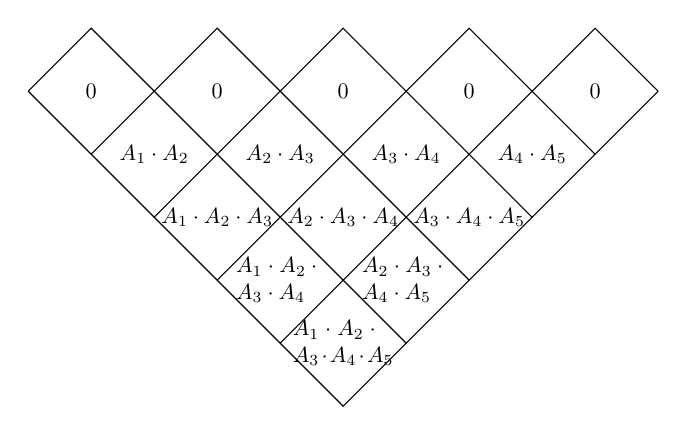
\begin{tikzpicture}[scale = 0.8, every node/.style={scale=0.8}]
    \draw (0,0) -- (5, -5) -- (10, 0)
          (0, 0) -- (1, 1) -- (6, -4)
          (1, -1) -- (3, 1) -- (7, -3)
          (2, -2) -- (5, 1) -- (8, -2)
          (3, -3) -- (7, 1) -- (9, -1)
          (4, -4) -- (9, 1) -- (10, 0);
    \draw (1, 0) node {$0$}
          (3, 0) node {$0$}
          (5, 0) node {$0$}
          (7, 0) node {$0$}
          (9, 0) node {$0$}
          (2, -1) node {$A_1 \cdot A_2$}
          (4, -1) node {$A_2 \cdot A_3$}
          (6, -1) node {$A_3 \cdot A_4$}
          (8, -1) node {$A_4 \cdot A_5$}
          (3, -2) node {$A_1 \cdot A_2 \cdot A_3$}
          (5, -2) node {$A_2 \cdot A_3 \cdot A_4$}
          (7, -2) node {$A_3 \cdot A_4 \cdot A_5$}
          (4, -3) node [text width=1.4cm] {$A_1 \cdot A_2 \cdot A_3 \cdot A_4$}
          (6, -3) node [text width=1.4cm] {$A_2 \cdot A_3 \cdot A_4 \cdot A_5$}
          (5, -4) node [text width=1.6cm] {$A_1 \cdot A_2 \cdot A_3 \cdot A_4 \cdot A_5$};
\end{tikzpicture}
\end{center}
\begin{tabular}{p{2cm} p{5cm} }
    \textbf{Sequence Alignment:} & You know how this works. Pull from the bottom diagonal. Assume a penalty of 1 for a mismatch and a penalty of 2 for a gap, use the dynamic programming algorithm to find an optimal alignment of the following sequences.
\end{tabular}\\
As an example from the last homework:
\begin{center}
    C C G G G T T A C C A\\
    G G A G T T C A
\end{center}
Show both the table and the optimal alignment.
\begin{center}
\begin{tabular}{|cc|c|c|c|c|c|c|c|c|c|c|c|c|}
    \hline
    & \textit{j} & 0 & 1 & 2 & 3 & 4 & 5 & 6 & 7 & 8 & 9 & 10 & 11\\
    \textit{i}& & C & C & G & G & G & T & T & A & C & C & A & \_\\
    \hline
    0 & G & \textbf{8} & \textbf{6} & 5 & 4 & 6 & 7 & 8 & 9 & 11 & 12 & 14 & 16\\
    \hline
    1 & G & 9 & 7 & \textbf{5} & 5 & 4 & 6 & 6 & 7 & 9 & 10 & 12 & 14\\
    \hline
    2 & A & 11 & 9 & \textbf{7} & 5 & 5 & 4 & 5 & 5 & 7 & 8 & 10 & 12\\
    \hline
    3 & G & 12 & 10 & 8 & \textbf{6} & \textbf{4} & 4 & 3 & 4 & 5 & 6 & 8 & 10\\
    \hline
    4 & T & 14 & 12 & 10 & 8 & 6 & \textbf{4} & 3 & 2 & 3 & 4 & 6 & 8\\
    \hline
    5 & T & 16 & 14 & 12 & 10 & 8 & 6 & \textbf{4} & 3 & 1 & 2 & 4 & 6\\
    \hline
    6 & C & 18 & 16 & 14 & 12 & 10 & 8 & 6 & \textbf{4} & \textbf{2} & \textbf{0} & 2 & 4\\
    \hline
    7 & A & 20 & 18 & 16 & 14 & 12 & 10 & 8 & 6 & 4 & 2 & \textbf{0} & 2\\
    \hline
    8 & \_ & 22 & 20 & 18 & 16 & 14 & 12 & 10 & 8 & 6 & 4 & 2 & \textbf{0}\\
    \hline
\end{tabular}
\end{center}

\section{Minimum Spanning Trees and Greedy Algorithms}
\begin{longtable}{p{2cm} p{5cm} }
    \textbf{Spanning Tree} & For a graph $G$, it's spanning tree is a connected subgraph that contains all of $G$'s verticies and is a tree.\\
    \textbf{Minimum}\\ \textbf{Spanning Tree} & For a graph $G$, it is a spanning tree of minimum weight.\\\\
    \textbf{Prim's}\\ \textbf{Algorithm} & Builds a minimum spanning tree vertex by vertex using an arbitrary starting vertex. Each step it will add the cheapest possible connection from the current vertex to the next. The algorithm is $\Theta(n^2)$.\\
    \textbf{Kruskal's}\\ \textbf{Algorithm} & \parbox[t]{5cm}{
    Builds a minimum spanning tree edge by edge, taking the cheapest edge available unless it causes a cycle. The steps to implement are as follows:
    \begin{enumerate}
        \item Sort the edges in time $\Theta(E \lg(E))$.
        \item Loop through the list of edges for a candidate edge. In worst case, it is $\Theta(E)$.
    \end{enumerate}
    In the worst case, though, every vertex is connected to every other vertex. This means $E \in \Theta(V^2)$. Thus, the worst case complexity is $\Theta((V^2 \lg(E))$.
    }
\end{longtable}
From the above descriptions, we can quickly conclude that Kruskal's Algorithm is better for sparse graphs, and Prim's Algorithm is better for dense graphs.
\newpage
\begin{longtable}{p{2cm} p{5cm} }
    \textbf{Dijkstra's}\\ \textbf{Algorithm} & \parbox[t]{5cm}{
    Builds a shortest path from a vertex $v_0$ to a destination $v_n$ vertex by vertex using an arbitrary starting vertex. Each step it will add the cheapest possible connection from the tree to another vertex, \textit{using the available connections already made in order to reduce possible costs}. The algorithm is $\Theta(n^2)$.
    }
\end{longtable}

\section{Backtracking}
Note that the book explicitly states that backtracking is a modification of DFS. We just DFS a lot.\\\\
\begin{longtable}{p{2.2cm} p{5cm} }
    \textbf{DFS} & DFS is a $\Theta(V + E)$ traversal of any graph. Pseudocode is as follows.\\
    \textbf{Backtracking} & Create a state space tree and traverse it. After determining that a node can only lead to death and destruction, go back to the parent and try again. The only way we can determine this is either by running out of options to come up with a solution, or using an upper bound to state a solution will get no worse. These algorithms are pretty terrible; the $n-queens$ problem uses a $\Theta(n^n)$ solution. The sum-of-subsets problem uses an upper bound and is a $T_n \approx 2^{n+1}-1$ algorithm
\end{longtable}
\section{Branch-and-Bound}
Note that the book explicitly states that backtracking is a modification of \textit{breadth}-first search. We just BFS a lot.\\\\
\begin{longtable}{p{2.2cm} p{5cm} }
    \textbf{BFS} & BFS is also a  $\Theta(V + E)$ traversal of any graph. Pseudocode is as follows.\\
    \textbf{Branch-and-Bound} & Just like Backtracking, with the modification that we visit the children of the current node only if its bound (an estimate guessing what will follow the current node) indicates that that path will lead to a better solution than the current best solution. That's the only effective difference. This is a \textbf{best}-first search.
\end{longtable}
\end{document}